\chapter{Reference Implementations}
\label{reference}

%%%%%%%%%%%%%%%%%%%%%%%%%%%%%%%%%%%%%%%%%%%%%%%%%%%%%%%%%%%%%%%%%%%%%%%%%%%%%%%%%%%%%%%%%%%

\section{Verilog reference implementations}

We have implemented Verilog cores for all instructions proposed in this
specification. These cores are permissively licensed under the ISC license and
can be obtained from \url{https://github.com/riscv/riscv-bitmanip/tree/master/verilog}.

\begin{figure}[t]
\begin{center}
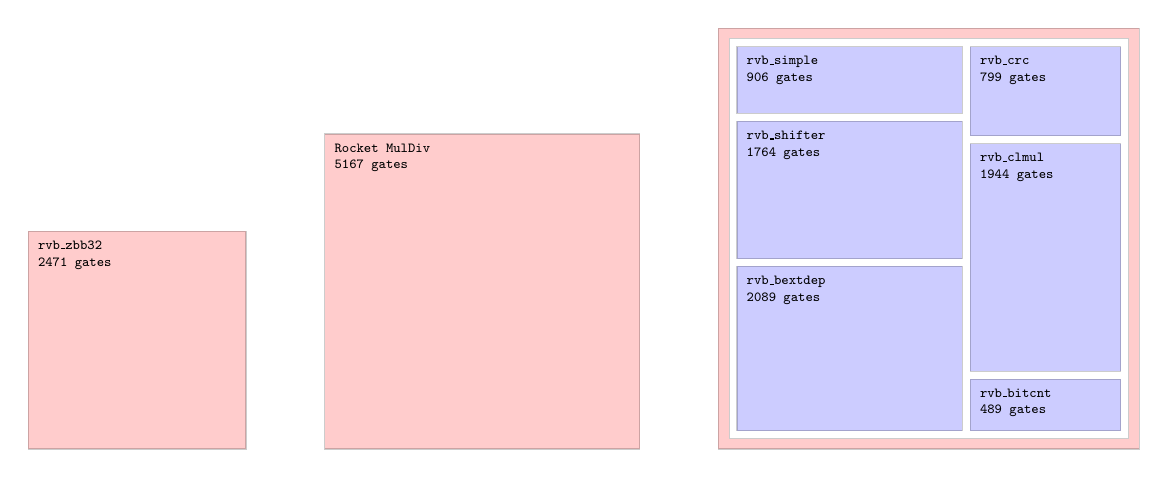
\begin{tikzpicture}
\draw [fill=red, opacity=0.2] (-5.000000,0) rectangle (-1,4.000000);
\node (label) at (-5.000000,4.000000) [below right, align=left, style={font=\tiny\tt}] {Rocket MulDiv \\ 5167 gates};
\draw [fill=red, opacity=0.2] (-8.766159,0) rectangle (-6.000000,2.766159);
\node (label) at (-8.766159,2.766159) [below right, align=left, style={font=\tiny\tt}] {rvb\_zbb32 \\ 2471 gates};
\draw [fill=red, opacity=0.2] (0,0) rectangle (5.343838,5.343838);
\draw [draw=black!20, fill=white] (0.134716,0.134716) rectangle (5.209123,5.209123);
\draw [draw=black, fill=blue, opacity=0.2] (0.234716,0.234716) rectangle (3.097199,2.318270);
\node (label) at (0.234716,2.318270) [below right, align=left, style={font=\tiny\tt}] {rvb\_bextdep \\ 2089 gates};
\draw [draw=black, fill=blue, opacity=0.2] (0.234716,2.418270) rectangle (3.097199,4.162114);
\node (label) at (0.234716,4.162114) [below right, align=left, style={font=\tiny\tt}] {rvb\_shifter \\ 1764 gates};
\draw [draw=black, fill=blue, opacity=0.2] (0.234716,4.262114) rectangle (3.097199,5.109123);
\node (label) at (0.234716,5.109123) [below right, align=left, style={font=\tiny\tt}] {rvb\_simple \\ 906 gates};
\draw [draw=black, fill=blue, opacity=0.2] (3.197199,0.234716) rectangle (5.109123,0.887341);
\node (label) at (3.197199,0.887341) [below right, align=left, style={font=\tiny\tt}] {rvb\_bitcnt \\ 489 gates};
\draw [draw=black, fill=blue, opacity=0.2] (3.197199,0.987341) rectangle (5.109123,3.879373);
\node (label) at (3.197199,3.879373) [below right, align=left, style={font=\tiny\tt}] {rvb\_clmul \\ 1944 gates};
\draw [draw=black, fill=blue, opacity=0.2] (3.197199,3.979373) rectangle (5.109123,5.109123);
\node (label) at (3.197199,5.109123) [below right, align=left, style={font=\tiny\tt}] {rvb\_crc \\ 799 gates};
\end{tikzpicture}
\end{center}
\caption{Area of 32-bit Rocket MulDiv core (center) compared to a complete implementation of all 32-bit instructions
proposed in this specification (right), and the 32-bit ``Zbb'' extension (left).}
\label{refhw32}
\end{figure}

For evaluation purposes we synthesized these cores for RV32 and RV64 to the following mockup ASIC cell library:

\begin{center}
\begin{tabular}{ll}
Cell & Gate Count \\
\hline
NOT   & 0.5 \\
NAND  & 1   \\
NOR   & 1   \\
XOR   & 3   \\
XNOR  & 3   \\
DFF   & 4   \\
\end{tabular}
\hfil
\begin{tabular}{ll}
Cell & Gate Count \\
\hline
AOI3  & 1.5 \\
OAI3  & 1.5 \\
AOI4  & 2   \\
OAI4  & 2   \\
NMUX  & 2.5 \\
MUX   & 3 \\
\end{tabular}
\end{center}

For comparison we also synthesized the rocket-chip MulDiv cores obtained using the following
rocket-chip configurations:

\begin{verbatim}
  class MulDivConfig64 extends Config(
      new WithFastMulDiv ++
      new DefaultConfig
  )

  class MulDivConfig32 extends Config(
      new WithRV32 ++
      new WithFastMulDiv ++
      new DefaultConfig
  )
\end{verbatim}

The following table lists the verilog reference cores and the instructions they implement:

\begin{center}
\begin{tabular}{lp{6cm}}
Module & Instructions \\
\hline
\tt rvb\_bextdep  & bext bdep grev gorc shfl unshfl                                               \\
\tt rvb\_clmul    & clmul clmulr clmulh                                                           \\
\tt rvb\_shifter  & sll srl sra slo sro rol ror fsl fsr slli.uw bset bclr binv bext bfp           \\
\tt rvb\_bmatxor  & bmatxor bmator                                                                \\
\tt rvb\_simple   & min max minu maxu andn orn xnor pack cmix cmov addiwu addwu subwu adduw subuw \\
\tt rvb\_bitcnt   & clz ctz pcnt bmatflip                                                         \\
\tt rvb\_crc      & crc32.[bhwd] crc32c.[bhwd]                                                    \\
\tt rvb\_full     & All of the above                                                              \\
\end{tabular}
\end{center}

On RV64 these cores also implement all {\tt *W} instruction variants of the above instructions.

Note that {\tt rvb\_shifter} also implements the base ISA {\tt sll}, {\tt srl},
and {\tt sra} instructions. Thus it can replace an existing implementation of
the base ISA shift instructions.

Fig.~\ref{refhw32} shows the area comparison for RV32 and fig.~\ref{refhw64} shows the comparison for RV64.
The area of the red frame surrounding the blue {\tt rvb\_*} modules accurately represents the added area
by the {\tt rvb\_full} wrapper module.

\begin{figure}[t]
\begin{center}
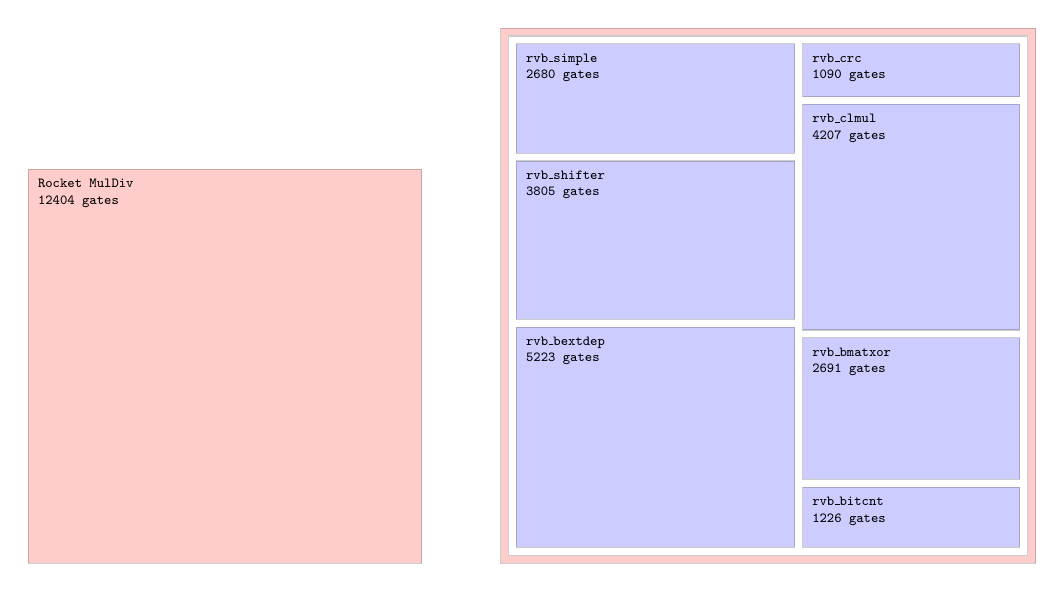
\begin{tikzpicture}
\draw [fill=red, opacity=0.2] (-6.000000,0) rectangle (-1,5.000000);
\node (label) at (-6.000000,5.000000) [below right, align=left, style={font=\tiny\tt}] {Rocket MulDiv \\ 12404 gates};
\draw [fill=red, opacity=0.2] (0,0) rectangle (6.792373,6.792373);
\draw [draw=black!20, fill=white] (0.099348,0.099348) rectangle (6.693025,6.693025);
\draw [draw=black, fill=blue, opacity=0.2] (0.199348,0.199348) rectangle (3.733225,2.996211);
\node (label) at (0.199348,2.996211) [below right, align=left, style={font=\tiny\tt}] {rvb\_bextdep \\ 5223 gates};
\draw [draw=black, fill=blue, opacity=0.2] (0.199348,3.096211) rectangle (3.733225,5.106601);
\node (label) at (0.199348,5.106601) [below right, align=left, style={font=\tiny\tt}] {rvb\_shifter \\ 3805 gates};
\draw [draw=black, fill=blue, opacity=0.2] (0.199348,5.206601) rectangle (3.733225,6.593025);
\node (label) at (0.199348,6.593025) [below right, align=left, style={font=\tiny\tt}] {rvb\_simple \\ 2680 gates};
\draw [draw=black, fill=blue, opacity=0.2] (3.833225,0.199348) rectangle (6.593025,0.963386);
\node (label) at (3.833225,0.963386) [below right, align=left, style={font=\tiny\tt}] {rvb\_bitcnt \\ 1226 gates};
\draw [draw=black, fill=blue, opacity=0.2] (3.833225,1.063386) rectangle (6.593025,2.859901);
\node (label) at (3.833225,2.859901) [below right, align=left, style={font=\tiny\tt}] {rvb\_bmatxor \\ 2691 gates};
\draw [draw=black, fill=blue, opacity=0.2] (3.833225,2.959901) rectangle (6.593025,5.824835);
\node (label) at (3.833225,5.824835) [below right, align=left, style={font=\tiny\tt}] {rvb\_clmul \\ 4207 gates};
\draw [draw=black, fill=blue, opacity=0.2] (3.833225,5.924835) rectangle (6.593025,6.593025);
\node (label) at (3.833225,6.593025) [below right, align=left, style={font=\tiny\tt}] {rvb\_crc \\ 1090 gates};
\end{tikzpicture}
\end{center}
\caption{Area of 64-bit Rocket MulDiv core (left) compared to a complete implementation of all 64-bit instructions
proposed in this specification (right).}
\label{refhw64}
\end{figure}

Regarding timing we evaluate the longest paths for {\tt rvb\_full} and
rocket-chip {\tt MulDiv}, measured in gate delays:

\begin{center}
\begin{tabular}{lcc}
& RV32 & RV64 \\
\hline
\tt rvb\_full & 30 & 57 \\
\tt MulDiv & 43 & 68 \\
\end{tabular}
\end{center}

All {\tt rvb\_*} reference cores provide single-cycle implementations of their functions,
with the exception of {\tt rvb\_clmul} which requires 4 cycles for a 32-bit
carry-less multiply and 8 cycles for a 64-bit carry-less multiply, and {\tt rvb\_crc}
which requires 1 cycle for each payload byte.

%%%%%%%%%%%%%%%%%%%%%%%%%%%%%%%%%%%%%%%%%%%%%%%%%%%%%%%%%%%%%%%%%%%%%%%%%%%%%%%%%%%%%%%%%%%

\section{Fast C reference implementations}
\label{fastc}

GCC has intrinsics for the bit counting instructions {\tt clz}, {\tt ctz}, and
{\tt pcnt}.  So a performance-sensitive application (such as an emulator)
should probably just use those:

\input{bextcref-fast-bitcnt}

For processors with BMI2 support GCC has intrinsics for bit extract and bit
deposit instructions (compile with {\tt -mbmi2} and include {\tt <x86intrin.h>}):

\input{bextcref-fast-bext-bmi2}

For other processors we need to provide our own implementations. The following
implementation is a good compromise between code complexity and runtime:

\input{bextcref-fast-bext}

For the other Bitmanip instructions the C reference functions given in Chapter~\ref{bext}
are already reasonably efficient.

%%%%%%%%%%%%%%%%%%%%%%%%%%%%%%%%%%%%%%%%%%%%%%%%%%%%%%%%%%%%%%%%%%%%%%%%%%%%%%%%%%%%%%%%%%%

\section{Bit permutation instructions as bit-index operations}

For programs that synthesize sequences of bit permutation instructions it can
be useful to describe bit permutation instructions in terms of bit-index
operations.

Expressed as bit-index operation, {\tt ror} is just subtraction and {\tt grev}
is just XOR:

\begin{minipage}{\linewidth}
\begin{verbatim}
  uint_xlen_t ror(uint_xlen_t a, uint_xlen_t b)
  {
    uint_xlen_t ret = 0;
    for (int i = 0; i < XLEN; i++) {
      int j = (i - b) & (XLEN-1);
      ret |= ((a >> i) & 1) << j;
    }
    return ret;
  }
\end{verbatim}
\end{minipage}

\begin{minipage}{\linewidth}
\begin{verbatim}
  uint_xlen_t grev(uint_xlen_t a, uint_xlen_t b)
  {
    uint_xlen_t ret = 0;
    for (int i = 0; i < XLEN; i++) {
      int j = (i ^ b) & (XLEN-1);
      ret |= ((a >> i) & 1) << j;
    }
    return ret;
  }
\end{verbatim}
\end{minipage}

The following {\tt unperm()} function calculates the new position
of bit {\tt i} after {\tt unshfl} by {\tt k}.

\begin{minipage}{\linewidth}
\begin{verbatim}
  int unperm(int k, int i)
  {
    return ((k + (i & k & ~(k<<1))) & ~k) |
           (i & ~(k | (k<<1))) | ((i>>1) & k);
  }
\end{verbatim}
\end{minipage}

This allows us to write {\tt shfl} and {\tt unshfl} in the following way.

\begin{minipage}{\linewidth}
\begin{verbatim}
  uint_xlen_t shfl(uint_xlen_t a, uint_xlen_t b)
  {
    uint_xlen_t ret = 0;
    for (int i = 0; i < XLEN; i++) {
      int j = unperm(b & (XLEN/2-1), i);
      ret |= ((a >> j) & 1) << i;
    }
    return ret;
  }
\end{verbatim}
\end{minipage}

\begin{minipage}{\linewidth}
\begin{verbatim}
  uint_xlen_t unshfl(uint_xlen_t a, uint_xlen_t b)
  {
    uint_xlen_t ret = 0;
    for (int i = 0; i < XLEN; i++) {
      int j = unperm(b & (XLEN/2-1), i);
      ret |= ((a >> i) & 1) << j;
    }
    return ret;
  }
\end{verbatim}
\end{minipage}
